% !TeX root = ../main.tex

\chapter{简介}

\section{研究背景}

地表形变的监测是了解地球内部物理过程的重要手段。
许多地球物理现象,如火山,地震等,都会伴随地表的形变。
地表形变携带着这些现象的信息,使我们进一步了解地球内部的演化过程。

在实际应用中,地表形变的监测是了解和预防地质灾害的重要方法。
近年来,地面沉降及其引发的次生灾害对各国的经济及社会发展造成越来越严重的损失。
然而,传统的形变监测手段难以满足当前监测的要求:
传统方法需要人工在有限的点上布设台站,需要人力长期参与,且某些条件恶劣的区域很难人工操作;
由于人力成本的限制,在大尺度的范围上很难布设足够密的台站,而过于稀疏的台站并不能满足监测的需求。

合成干涉孔径雷达(Interferometric Synthetic Aperture Radar,InSAR)监测
具有成本低,覆盖范围广,全天候,非接触等优良特点。
而且相较于GPS,InSAR在垂直方向的能提供更高的精度,
目前已在地表沉降监测方面广泛应用,且取得了突出的成果。

\section{研究区域}

2008年7月16日,美国新墨西哥州阿蒂西亚(Artesia, New Mexico)东南部的一个卤水井(JWS Sinkhole)发生坍塌事件。
2008年11月3日,该区域离上述卤水井较近的另一卤水井(Loco Hills Sinkhole)同样发生了垮塌。
两次时间和空间均相近的坍塌引起了广泛的关注。
并且,离阿蒂西亚较近的卡尔斯巴德(Carlsbad)有一卤水井,并且当地的地质背景和以上两个坍塌的卤水井类似。
三个卤水井的位置如图\ref{fig:carlsbad}所示。
和以上二者不同的是,此卤水井位于市区,和两条重要的高速公路相邻,如果发生坍塌,会造成更严重的伤害和经济损失。
为了避免此种情况发生,从2009年八月份开始,当地相关部门就陆续使用地震学,地电学等的方法对此地展开地质勘探。
从2012年开始,当地政府部门展开修复工作。

本文的研究区域即为卡尔斯巴德的卤水井,本文检测该区域的地表形变,并对该形变建立合适的物理模型。

\begin{figure}[htb]
  \centering
  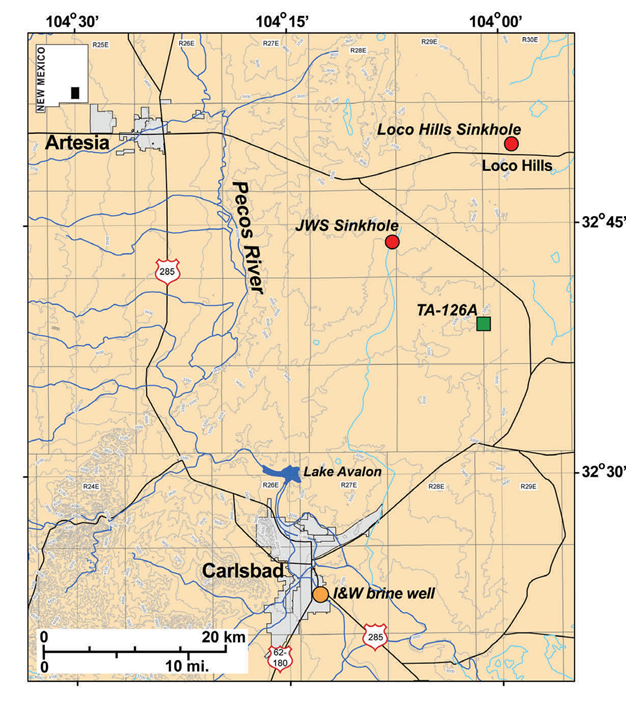
\includegraphics[width=0.8\textwidth]{carlsbad.png}
  \caption{新墨西哥州的卤水井}
  \label{fig:carlsbad}
  \note{注:图中JWS Sinkhole和Loco Hills Sinkhole为已经坍塌的卤水井,I\&W Brine Well为未坍塌的卤水井,也是本文的研究区域。}
\end{figure}

\section{研究意义}

地面沉降是一种危害严重的自然灾害,具有分布范围广,持续时间长的特点。
合成孔径雷达干涉技术(InSAR)技术,具有大尺度观测的特点,且不需要任何地面上的人工操作,
能对同一区域进行重复的卫星观测,而且测得的形变较为精密,能很好地满足地面沉降检测的要求,
从而对突发灾害作出预报。

我国某些区域尤其是矿产资源比较丰富的地区,同面面临着坍塌的风险。
本研究所使用的方法,可以对此类灾害起到一定的预警作用。

\section{本研究的主要内容}

\subsection{使用SBAS-InSAR技术获取当地地表形变}

本研究选取该卤水井所在区域(约1km×1km)ALOS 1(Advanced Land Observation Satellite 1)从2007年到2011年的15幅影像,
通过SBAS-InSAR技术获取当地地表形变以及平均的形变速率。这一步使用的软件为StamPS。

\subsection{使用mogi模型对该形变建模}

首先观察SBAS-InSAR得到的形变特征,选取比较合适的mogi模型,对该形变进行理论建模,
建模所使用的软件为GBIS。
然后与已有的研究成果相对比,并结合当地地质背景,分析所得模型的可靠程度。

\section{本研究的组织结构}

本研究的组织结构如图\ref{fig:flow}所示:

\begin{figure}[htb]
  \centering
  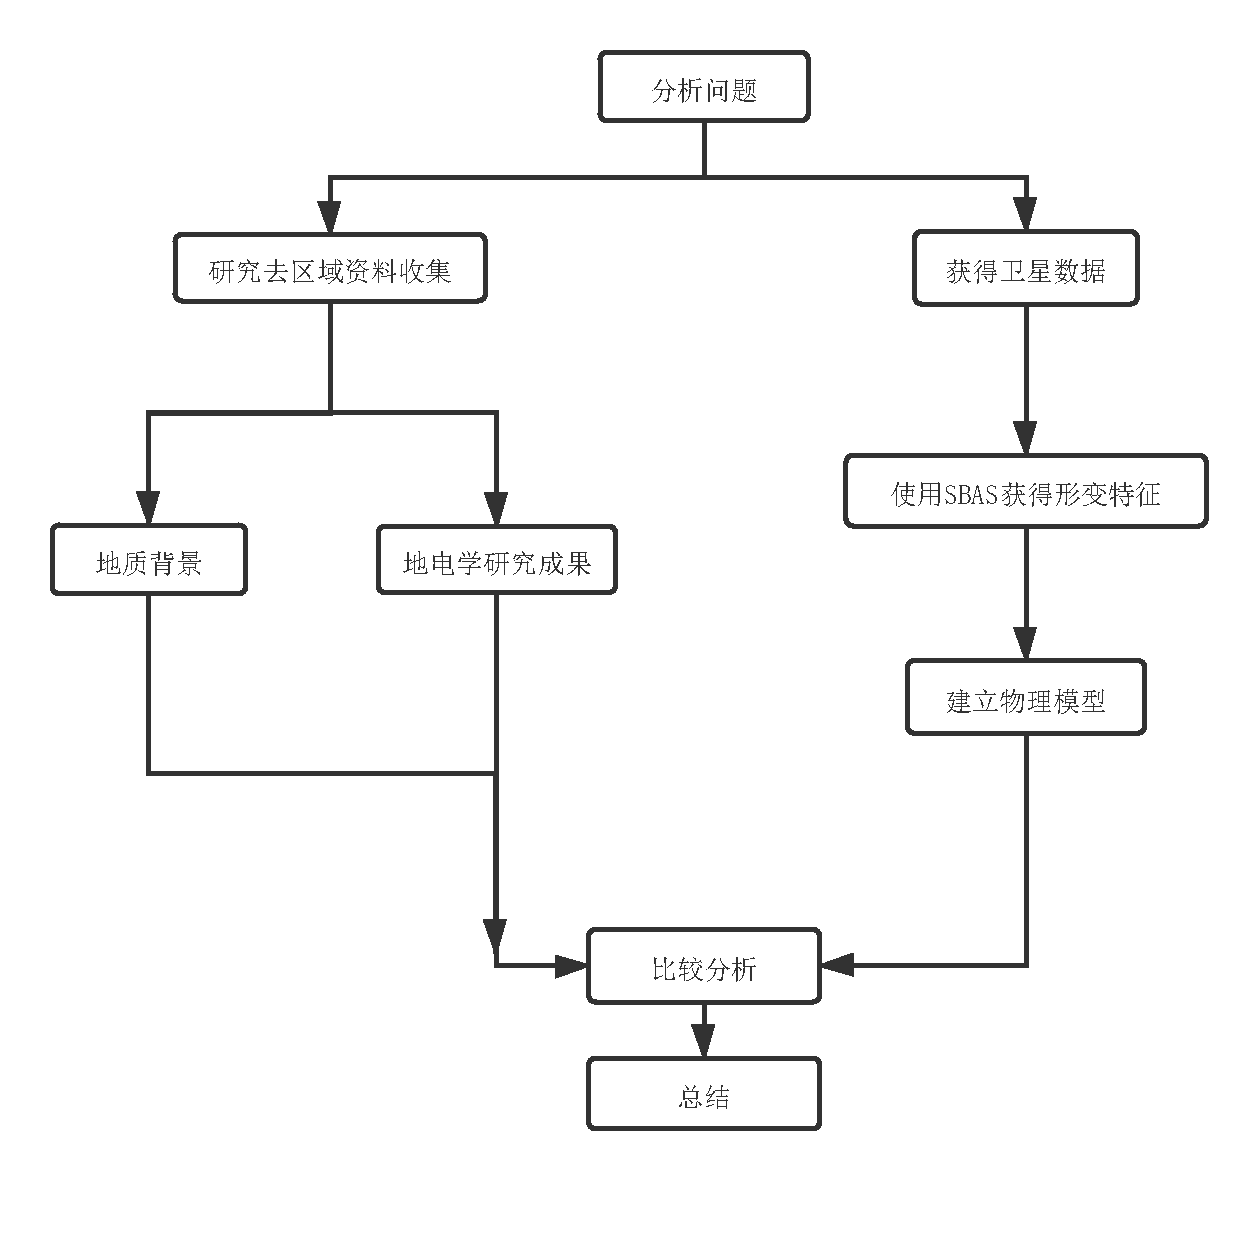
\includegraphics[width=0.8\textwidth]{flow.pdf}
  \caption{本研究的组织结构}
  \label{fig:flow}
\end{figure}